\chapter{Experimental Setup}
\section{Synchrotron Radiation}
The radiation emitted by a relativistic charged particle accelerated to a circular orbit inside a magnetic field is called synchrotron radiation. The radiation is emitted tangential to the circular movement of the charged particle and covers a broad spectral range. Given all the fundamental and experimental parameters are known, the radiation can be calculated exactly based on classical electrodynamics. The theory specific for synchrotron radiation was developed by Schwinger \cite{schwinger_classical_1949}. A comprehensive summary can be found in \cite{munro_chapter_1987}, for example.

The total emitted radiant power $P$ by each relativistic electron is
\begin{align}
 P = \frac{1}{4 \pi \gls{epsilon_0}} \frac{2}{3} \frac{\gls{e}^2 \gls{c}}{R^2}\Big( \frac{E}{\gls{m_0} \gls{c}^2}\Big)^4 \text{,}
\end{align}
where \gls{e} is the elementary charge, \gls{c} is the speed of light in vacuum, $E$ is the particles energy, \gls{m_0} is the rest mass of the particle and $R$ is the radius of the circular trajectory imposed by the magnetic field.

\Gls{mls} \cite{brandt_metrology_2007} of \gls{ptb}
\Gls{bessy}
Schwinger equation \cite{schwinger_classical_1949}
Primary source standard \cite{thornagel_electron_2001}
description \cite{munro_chapter_1987}
\begin{figure}
 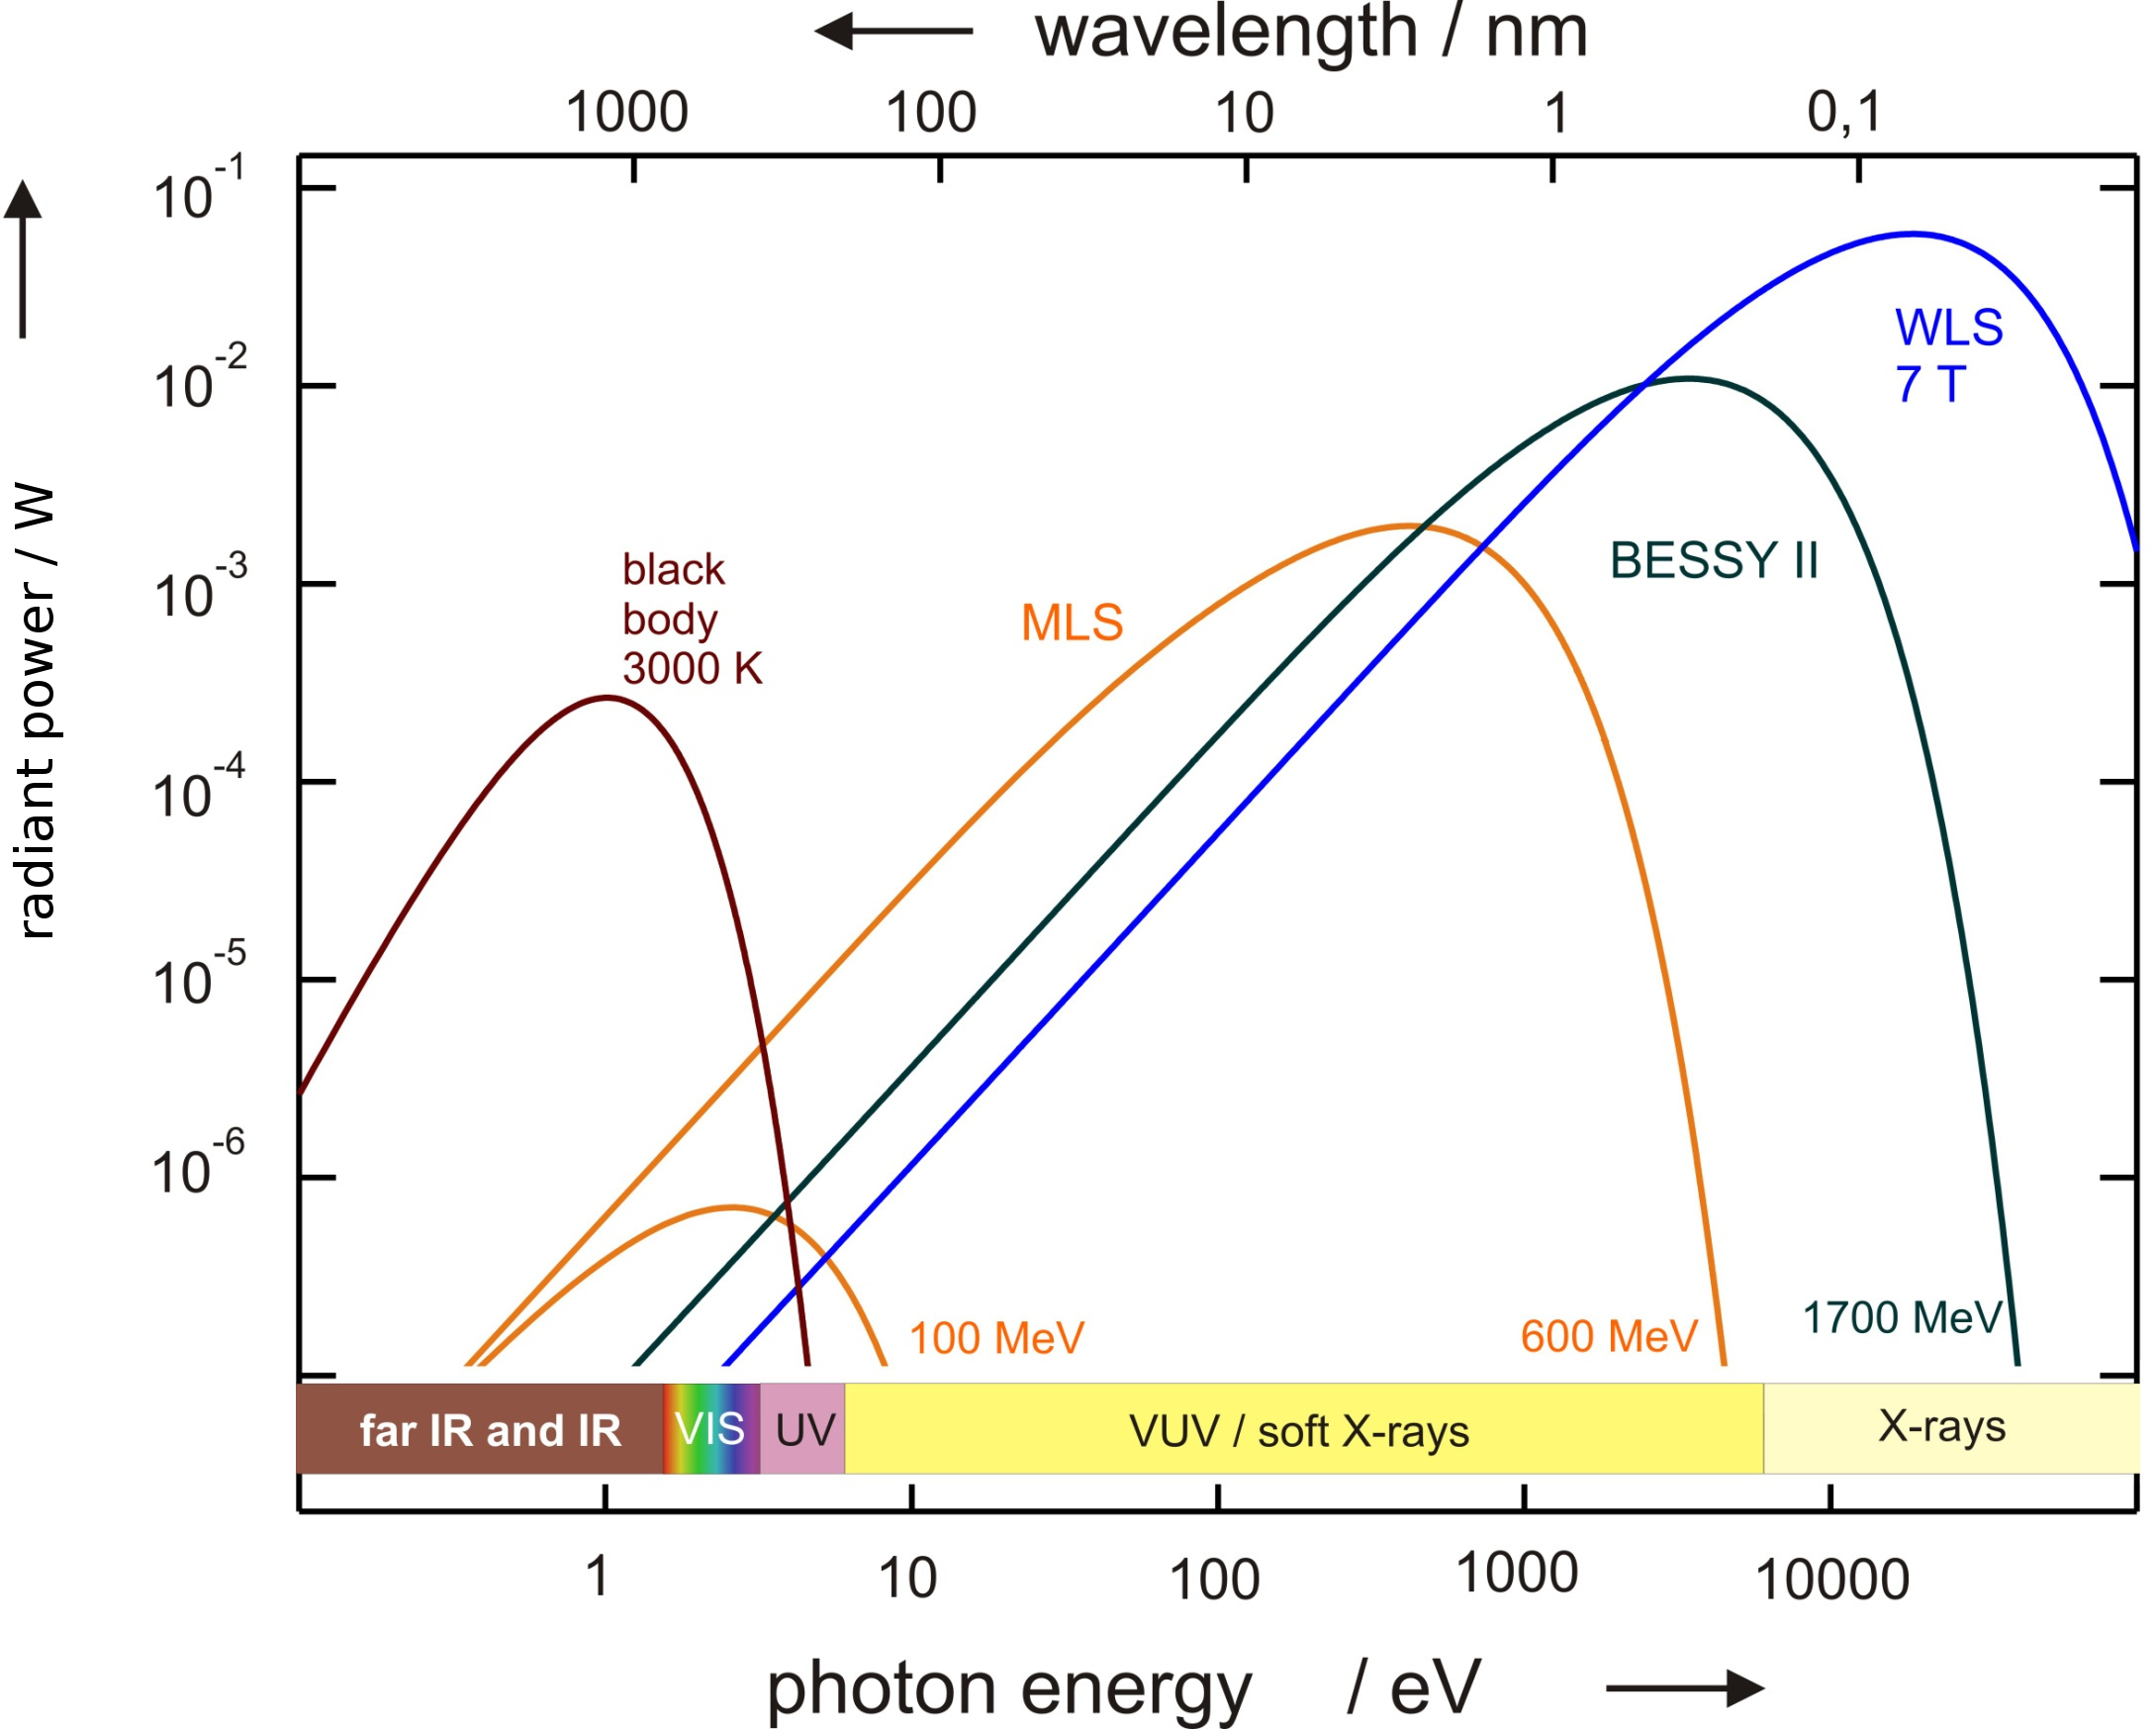
\includegraphics[width=0.7\textwidth]{img/exp-bessy-dipole-spectrum.jpeg}
 \caption[Experimental synchrotron radiation spectra]{Experimental synchrotron radiation spectra for the \gls{mls} and \gls{bessy} in comparison to black body radiation\footnote{Image taken from Beckhoff et al.~\cite{beckhoff_quarter-century_2009}}.}
 \label{ch_exp:fig_experimental_synchrotron_spectra}
\end{figure}


\section{The SX700 and EUVR Beamlines}
\begin{figure*}[htb]
    \def\svgwidth{\textwidth}
    \import{svg/}{exp-ptb-beamlines.pdf_tex}
    \caption[\Gls{ptb} Beamlines in the \gls{bessy} laboratory.]{Beamlines in the laboratory at \gls{bessy}.}
    \label{ch_exp:fig_beamlines_bessy}
\end{figure*}
SX700 \cite{beckhoff_quarter-century_2009}
\section{The ELLI and BigRef Reflectometers}
BigRef \cite{scholze_high-accuracy_2001}
ELLI \cite{soltwisch_polarization_2015}
\section{Grazing-incidence X-ray Fluorescence at the FCM Beamline}